\documentclass[a4paper, amsfonts, amssymb, amsmath, reprint, showkeys, nofootinbib, twoside]{revtex4-1}
\usepackage[english]{babel}
\usepackage[utf8]{inputenc}
\usepackage[colorinlistoftodos, color=green!40, prependcaption]{todonotes}
\usepackage[pdftex, pdftitle={Article}, pdfauthor={Author}]{hyperref}
\usepackage{amsthm}
\usepackage{mathtools}
\usepackage{physics}
\usepackage{xcolor}
\usepackage{caption}
\usepackage{hyperref}
\usepackage{multirow}
\usepackage{amsmath}
\usepackage{amssymb}
\usepackage{graphicx}
\graphicspath{Images}
\usepackage[left=23mm,right=13mm,top=35mm,columnsep=15pt]{geometry} 
\usepackage{adjustbox}
\usepackage{placeins}
\usepackage[T1]{fontenc}
\usepackage{float}
%\usepackage{longtable}
\usepackage{csquotes}
\usepackage{refstyle}
\usepackage{lipsum}
\usepackage{booktabs}

\begin{document}

\title{Study of Gamma-Gamma Coincidence using $^{22}\text{Na}$}
\author{Swaroop Ramakant Avarsekar}
\email{swaroop.avarsekar@niser.ac.in}
\affiliation{School of Physical Sciences, National Institute of Science Education and Research, HBNI, Jatni -752050, India}
\date{\today}

\begin{abstract}
Gamma gamma coincidence is phenomena when two gamma rays emitted from $^{22}\text{Na}$ are detected simultaneously used in identifying the radioactive isotope. $^{22}\text{Na}$ has a photopeak at 0.511 MeV due to positron annihilation and high energy peak at 1275 MeV. Two other peaks are also observed due to Compton scattering. It was seen that the coincidence rate is maximum for orientation of two detectors at $180^{\circ}$ and almost nil at zero degrees. Lower count rate at angles nearby $180^{\circ}$ is observed.
\end{abstract}

\keywords{Bremsstrahlung, Photo-peak, Coincidence}
\maketitle
\section{Theory}
\begin{figure}[H]
	\centering
	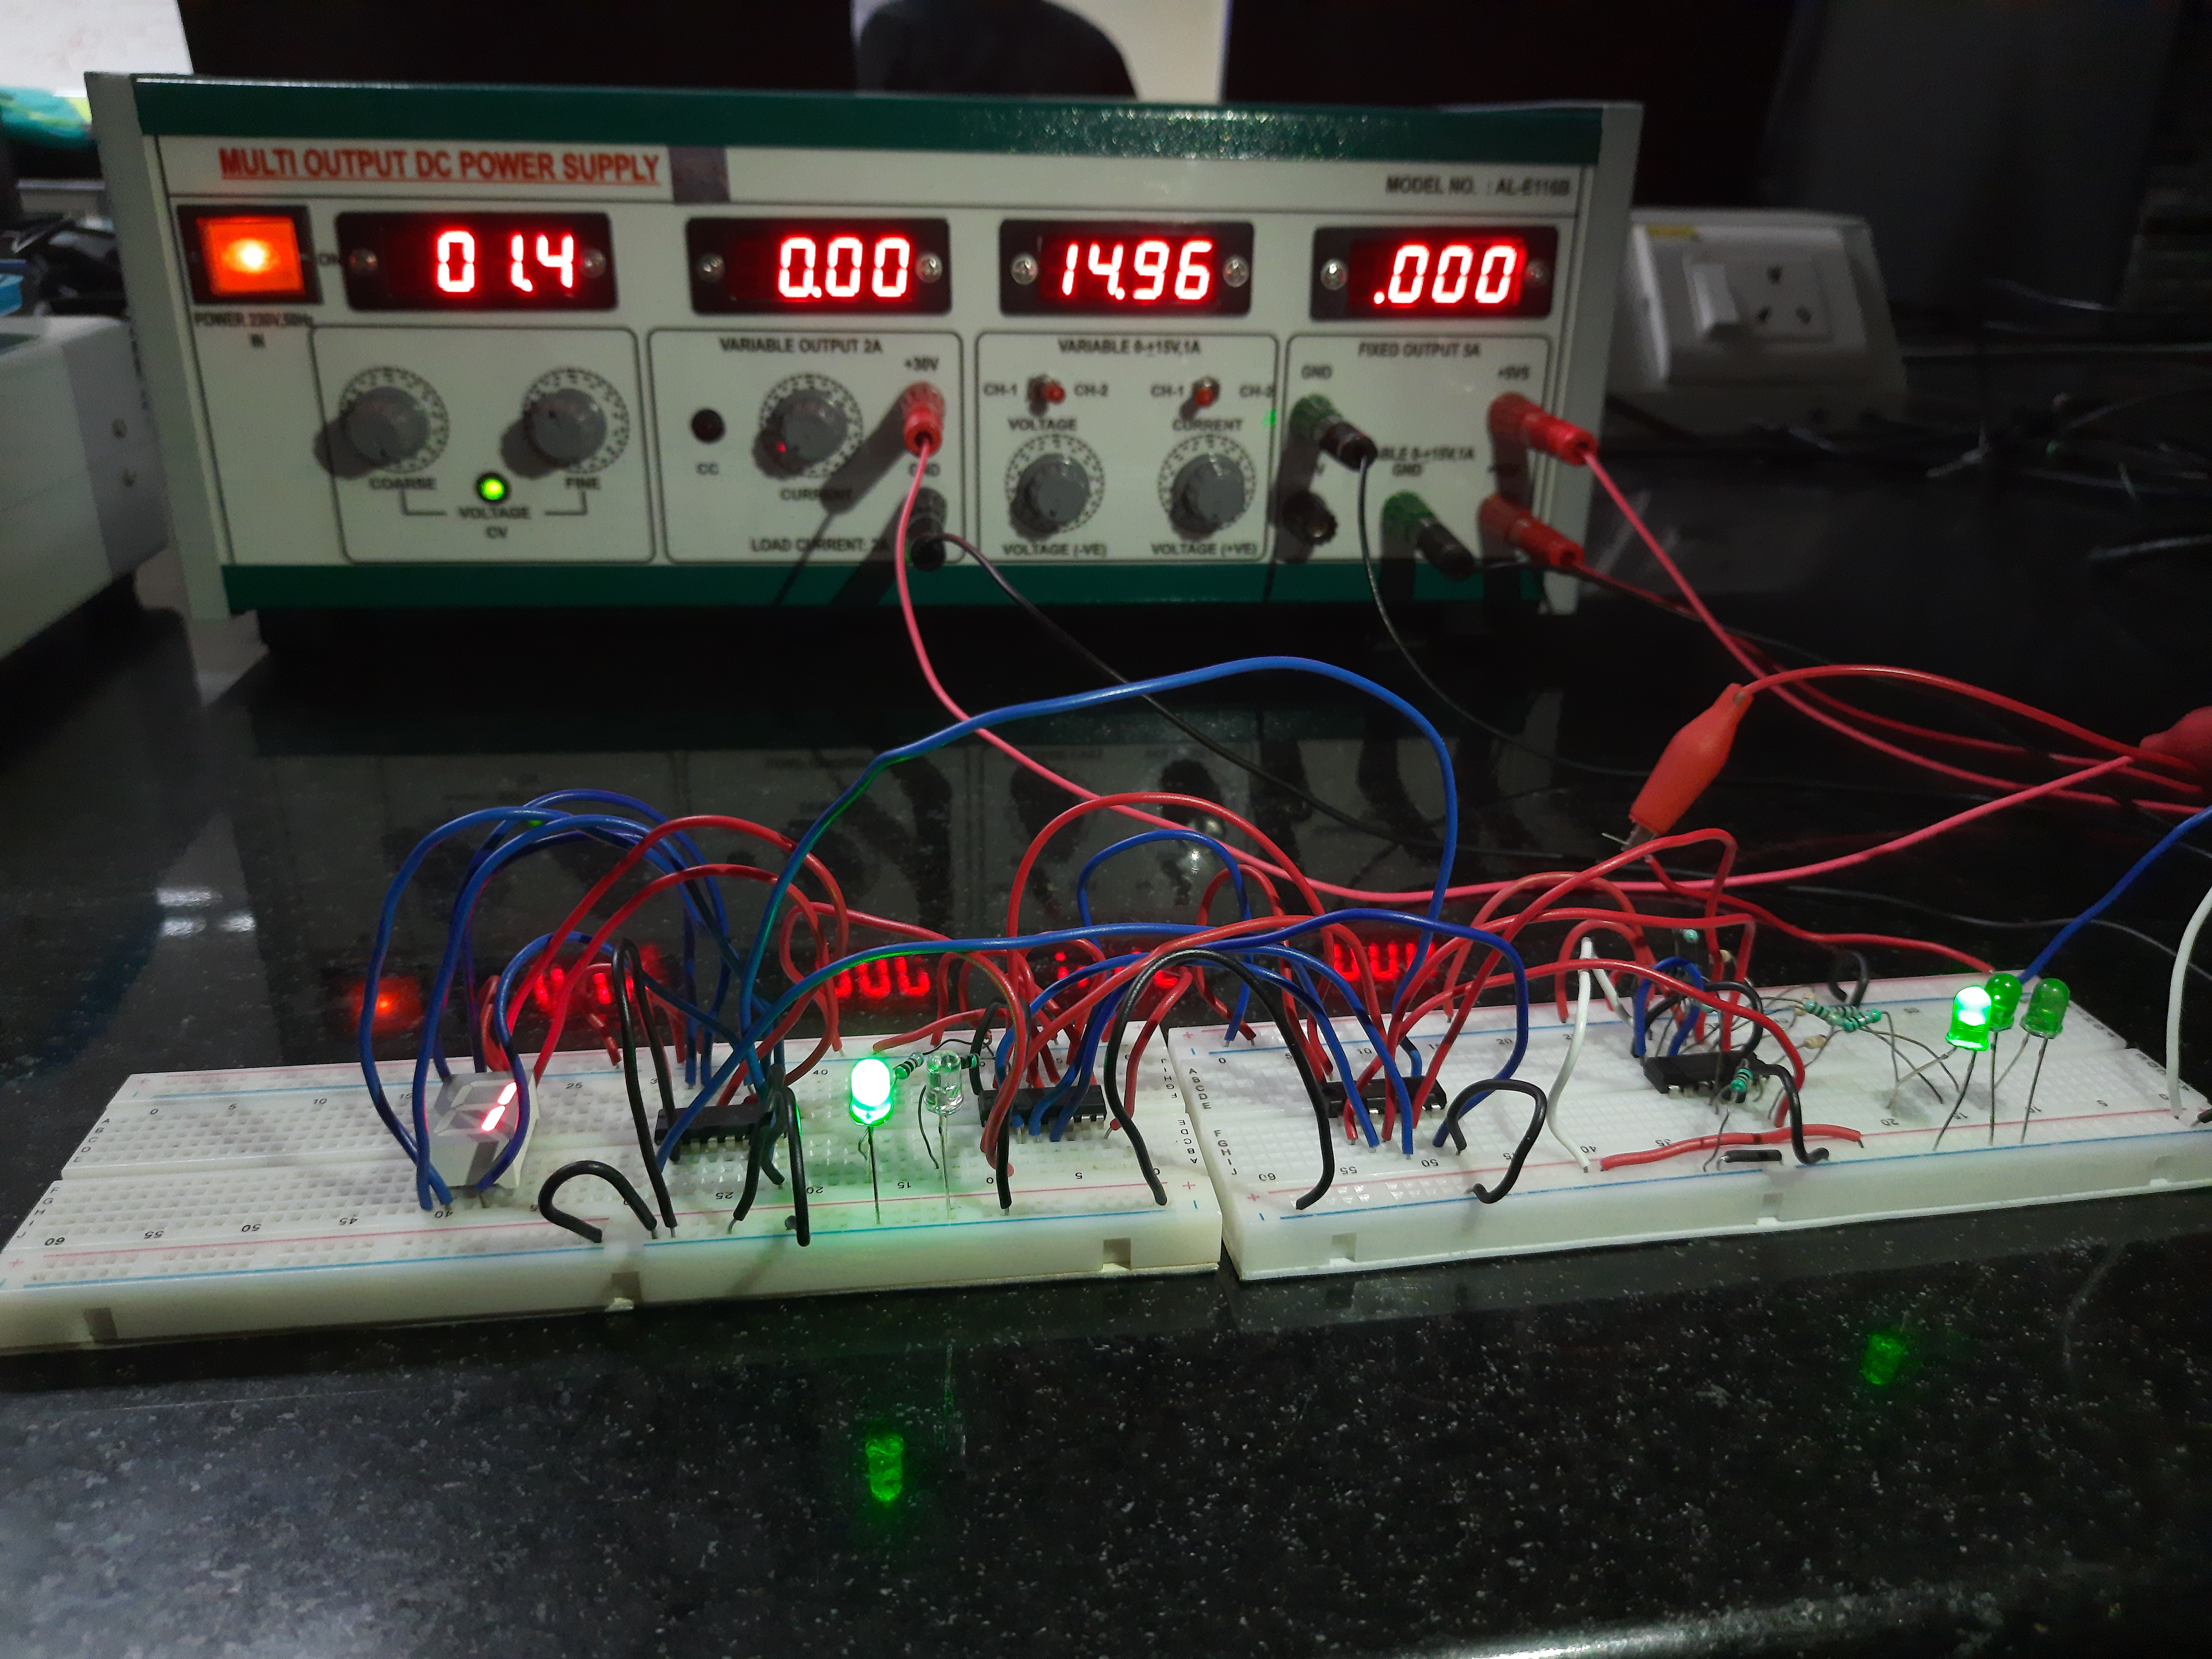
\includegraphics[scale=0.4]{1} 
	\caption{$^{22}\text{Na}$ decay scheme}
	\label{s}
\end{figure}

$^{22}\text{Na}$ is a radioactive isotope with a half life of 2.6 years. $^{22}\text{Na}$ decays to an excited state of $^{22}\text{Ne}$ by emission of a positron(90\%) or by electron capture(10\%). The excited $^{22}\text{Ne}$ produced has a mean life of 3 pico seconds
and emits 1.275 MeV. The positrons are emitted maxi- mum kinetic energy of 0.511 MeV. Positrons lose energy in the order of nano seconds.

The gamma rays emitted by energy conservation should have same energy conservation and by momentum conservation should have net momentum equal to  initial momentum of the positron. Gamma rays emitted by energy conservation should have same energy and net momentum equal to positron. In the rest frame of the positron,  it had no initial momentum and hence the two gamma rays must have equal and opposite momenta, measured in scintillation detector, at angles $180^{\circ}$, $90^{\circ}$ and two angles near $180^{\circ}$.

We also obtain heatmap with the data collected which includes 4 peaks due to photo-peaks, Compton scattering, and Bremsstrahlung. Photopeaks are due to gamma ray transfer, the incident gamma ray photon is deflected through an angle. The photon transfers a portion of its energy to the recoil electron. The energy transferred to the recoil electron can vary from zero to energy of the incident gamma ray energy, Bremsstrahlung is electromagnetic radiation produced by a sudden slowing down or deflection of charged particles. We may also observe peaks due to backscattering, coincidence peaks, annihilation peaks etc.

\section{Experiment}
A gamma detector consists of a scintillator integrated with a device capable of measuring the quanta of scintillation photons emitted from it as a result of an incident gamma. This scintillator is fused in pn junction in reverse bias.The depletion region thus created acts as an ionisation medium which converts the scintillation photons into a corresponding number of electron-hole pairs. The small amount of charge generated as a result of one gamma ray depositing its entire energy in the scintillator which then gets converted into a charge pulse by the PN junction results in an event in the photopeak region. Other interactions such as Compton scattering is also detected. The charge is fed to signal processing unit which amplifies and shapes the signal. Multi channel analyser with 1024 channels, detects, sorts and does the post processing. We put threshold of 100 channels as other are not required.

\begin{figure}[H]
	\centering
	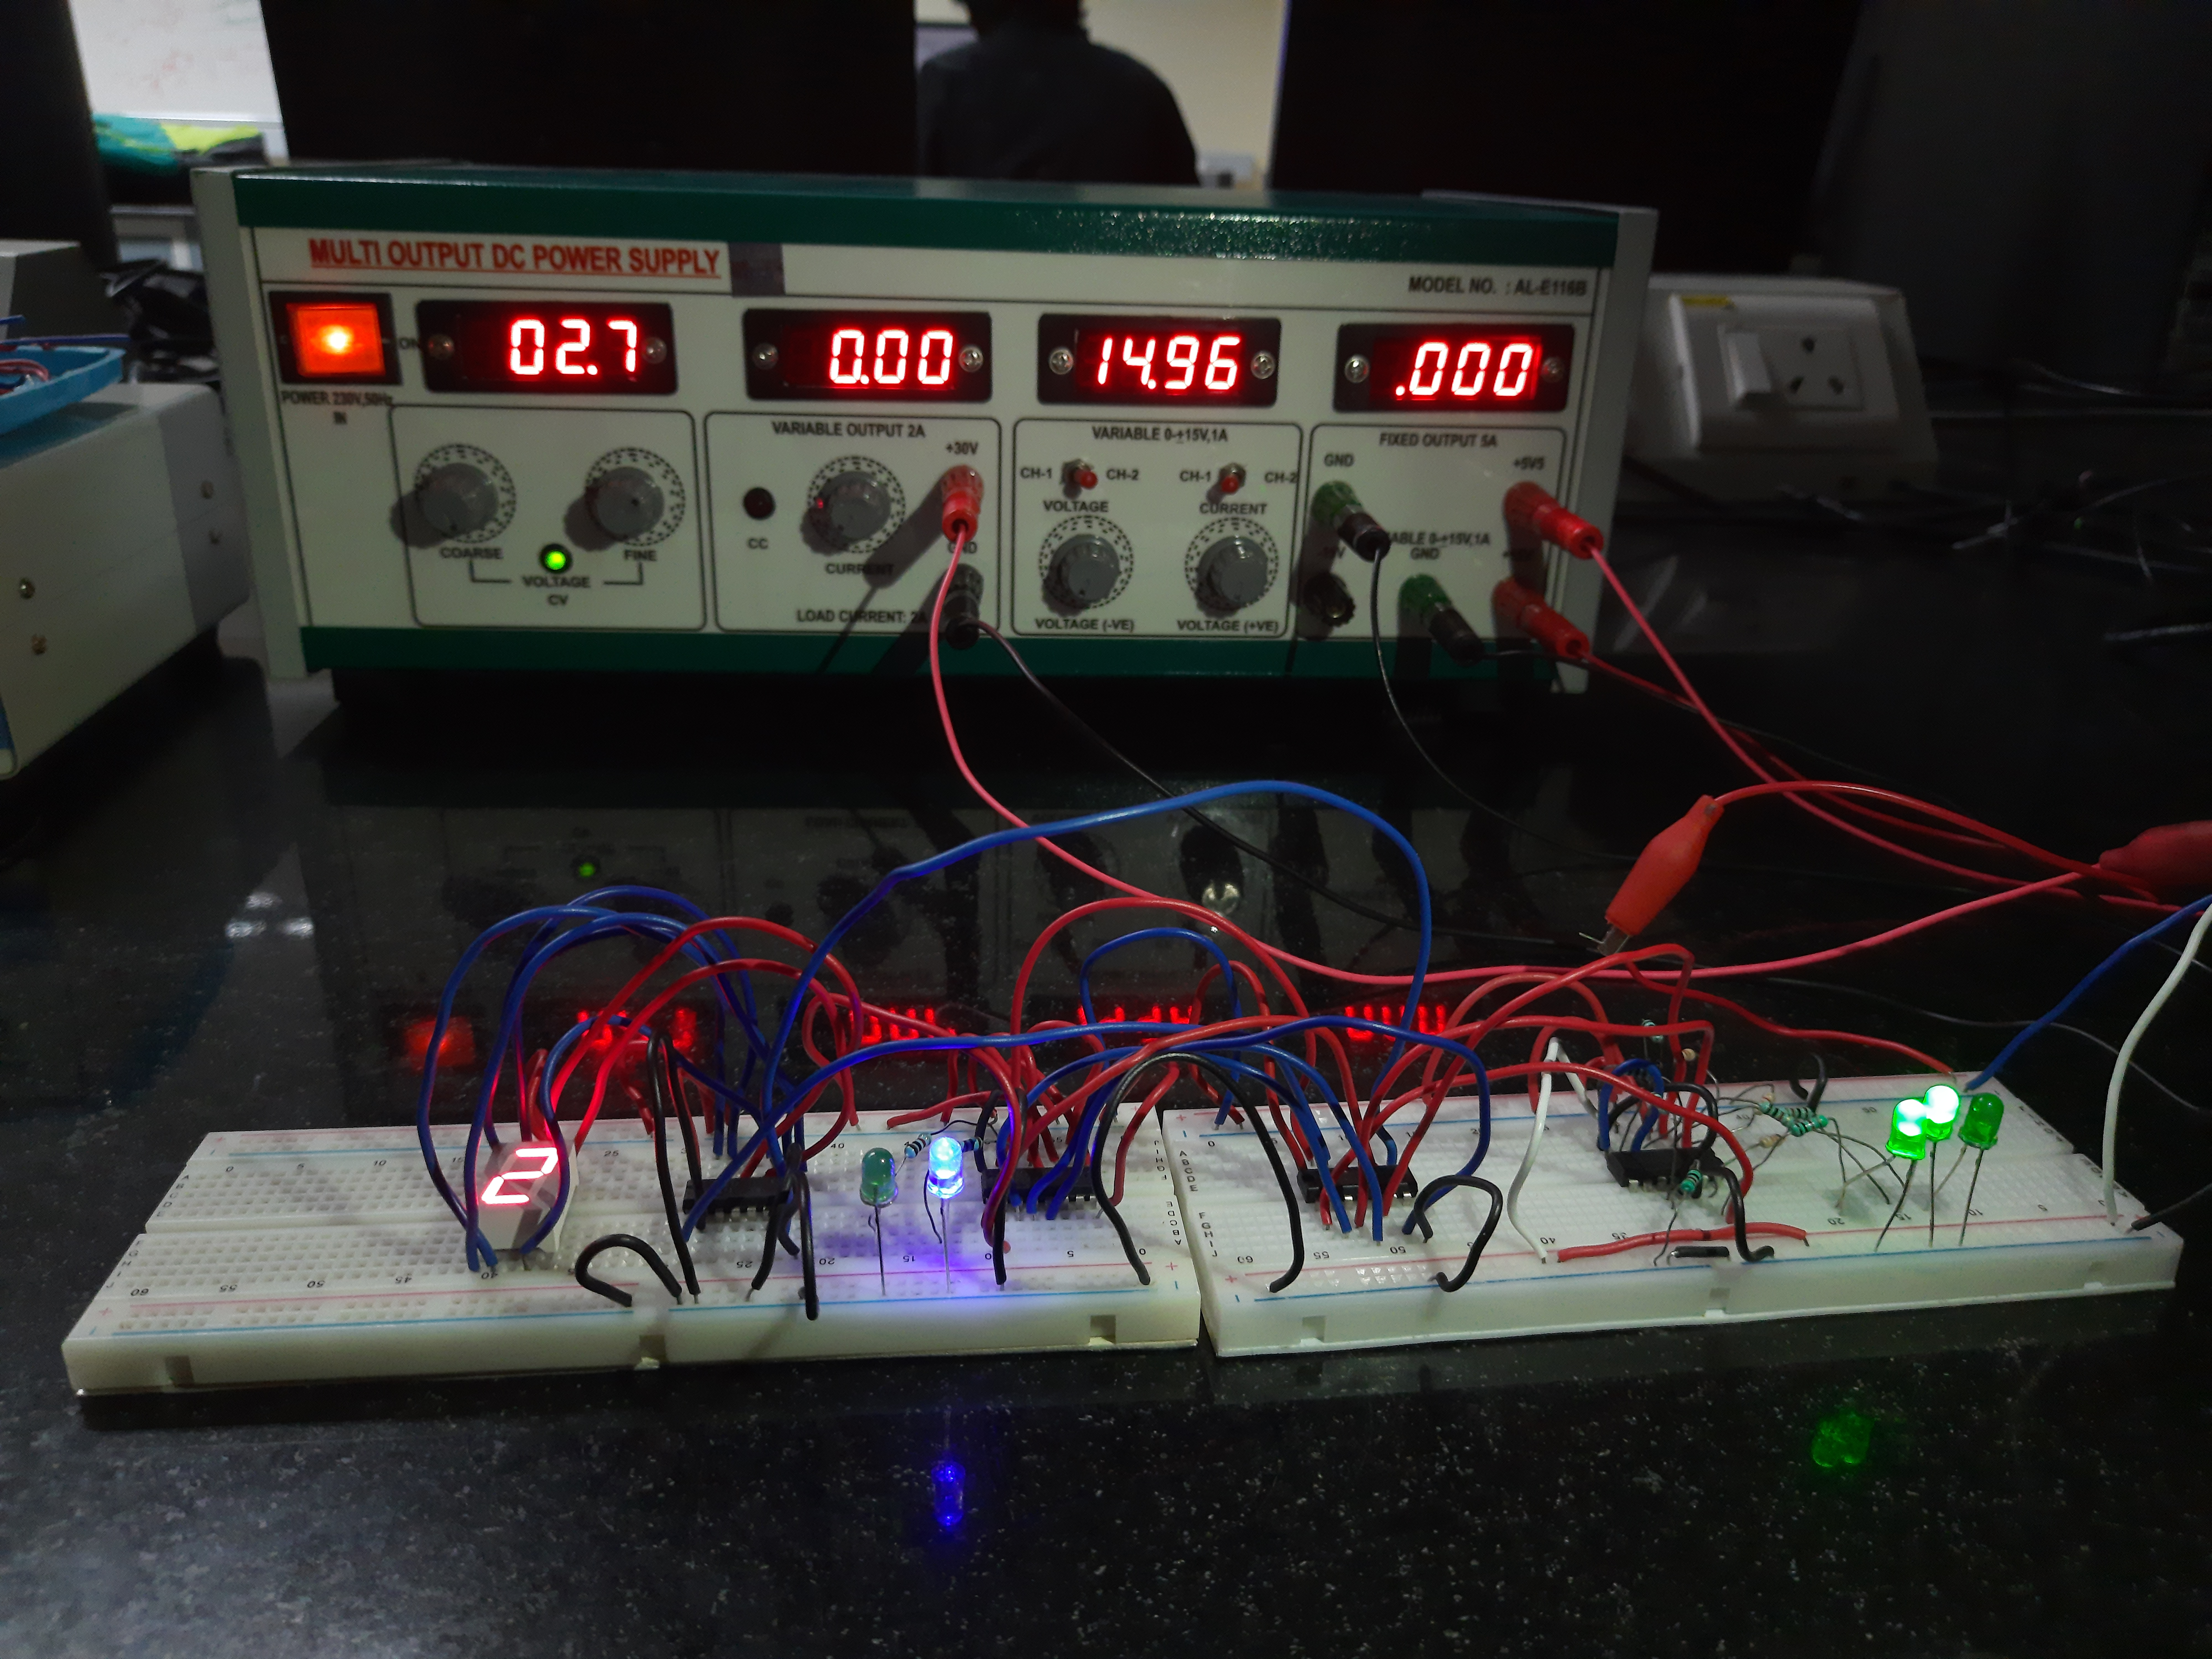
\includegraphics[scale=0.06]{2} 
	\caption{Experimental setup}
	\label{s}
\end{figure}

\begin{figure}[H]
	\centering
	\includegraphics[scale=0.4]{180} 
	\caption{3D heat map for 180 degrees }
	\label{s}
\end{figure}

\begin{table}[H]
	\centering
	\caption{Coincidence Count}
	\label{tab:my-table}
	\resizebox{\columnwidth}{!}{%
		\begin{tabular}{|c|c|c|}
			\hline
			Angle (deg) & Coincidence Count & Count Rate \\ \hline
			180         & 1238              & 0.3438     \\ \hline
			90          & 9                 & 0.0025     \\ \hline
			175         & 1103              & 0.3063     \\ \hline
			185         & 1104              & 0.3066     \\ \hline
		\end{tabular}%
	}
\end{table}

\begin{figure}[H]
	\centering
	\includegraphics[scale=0.4]{185} 
	\caption{3D heat map for 185 degrees }
	\label{s}
\end{figure}

\begin{figure}[H]
	\centering
	\includegraphics[scale=0.38]{175} 
	\caption{3D heat map for 175 degrees }
	\label{s}
\end{figure}

\begin{figure}[H]
	\centering
	\includegraphics[scale=0.34]{90} 
	\caption{3D heat map for 90 degrees }
	\label{s}
\end{figure}

\begin{figure*}[ht]
	\centering
	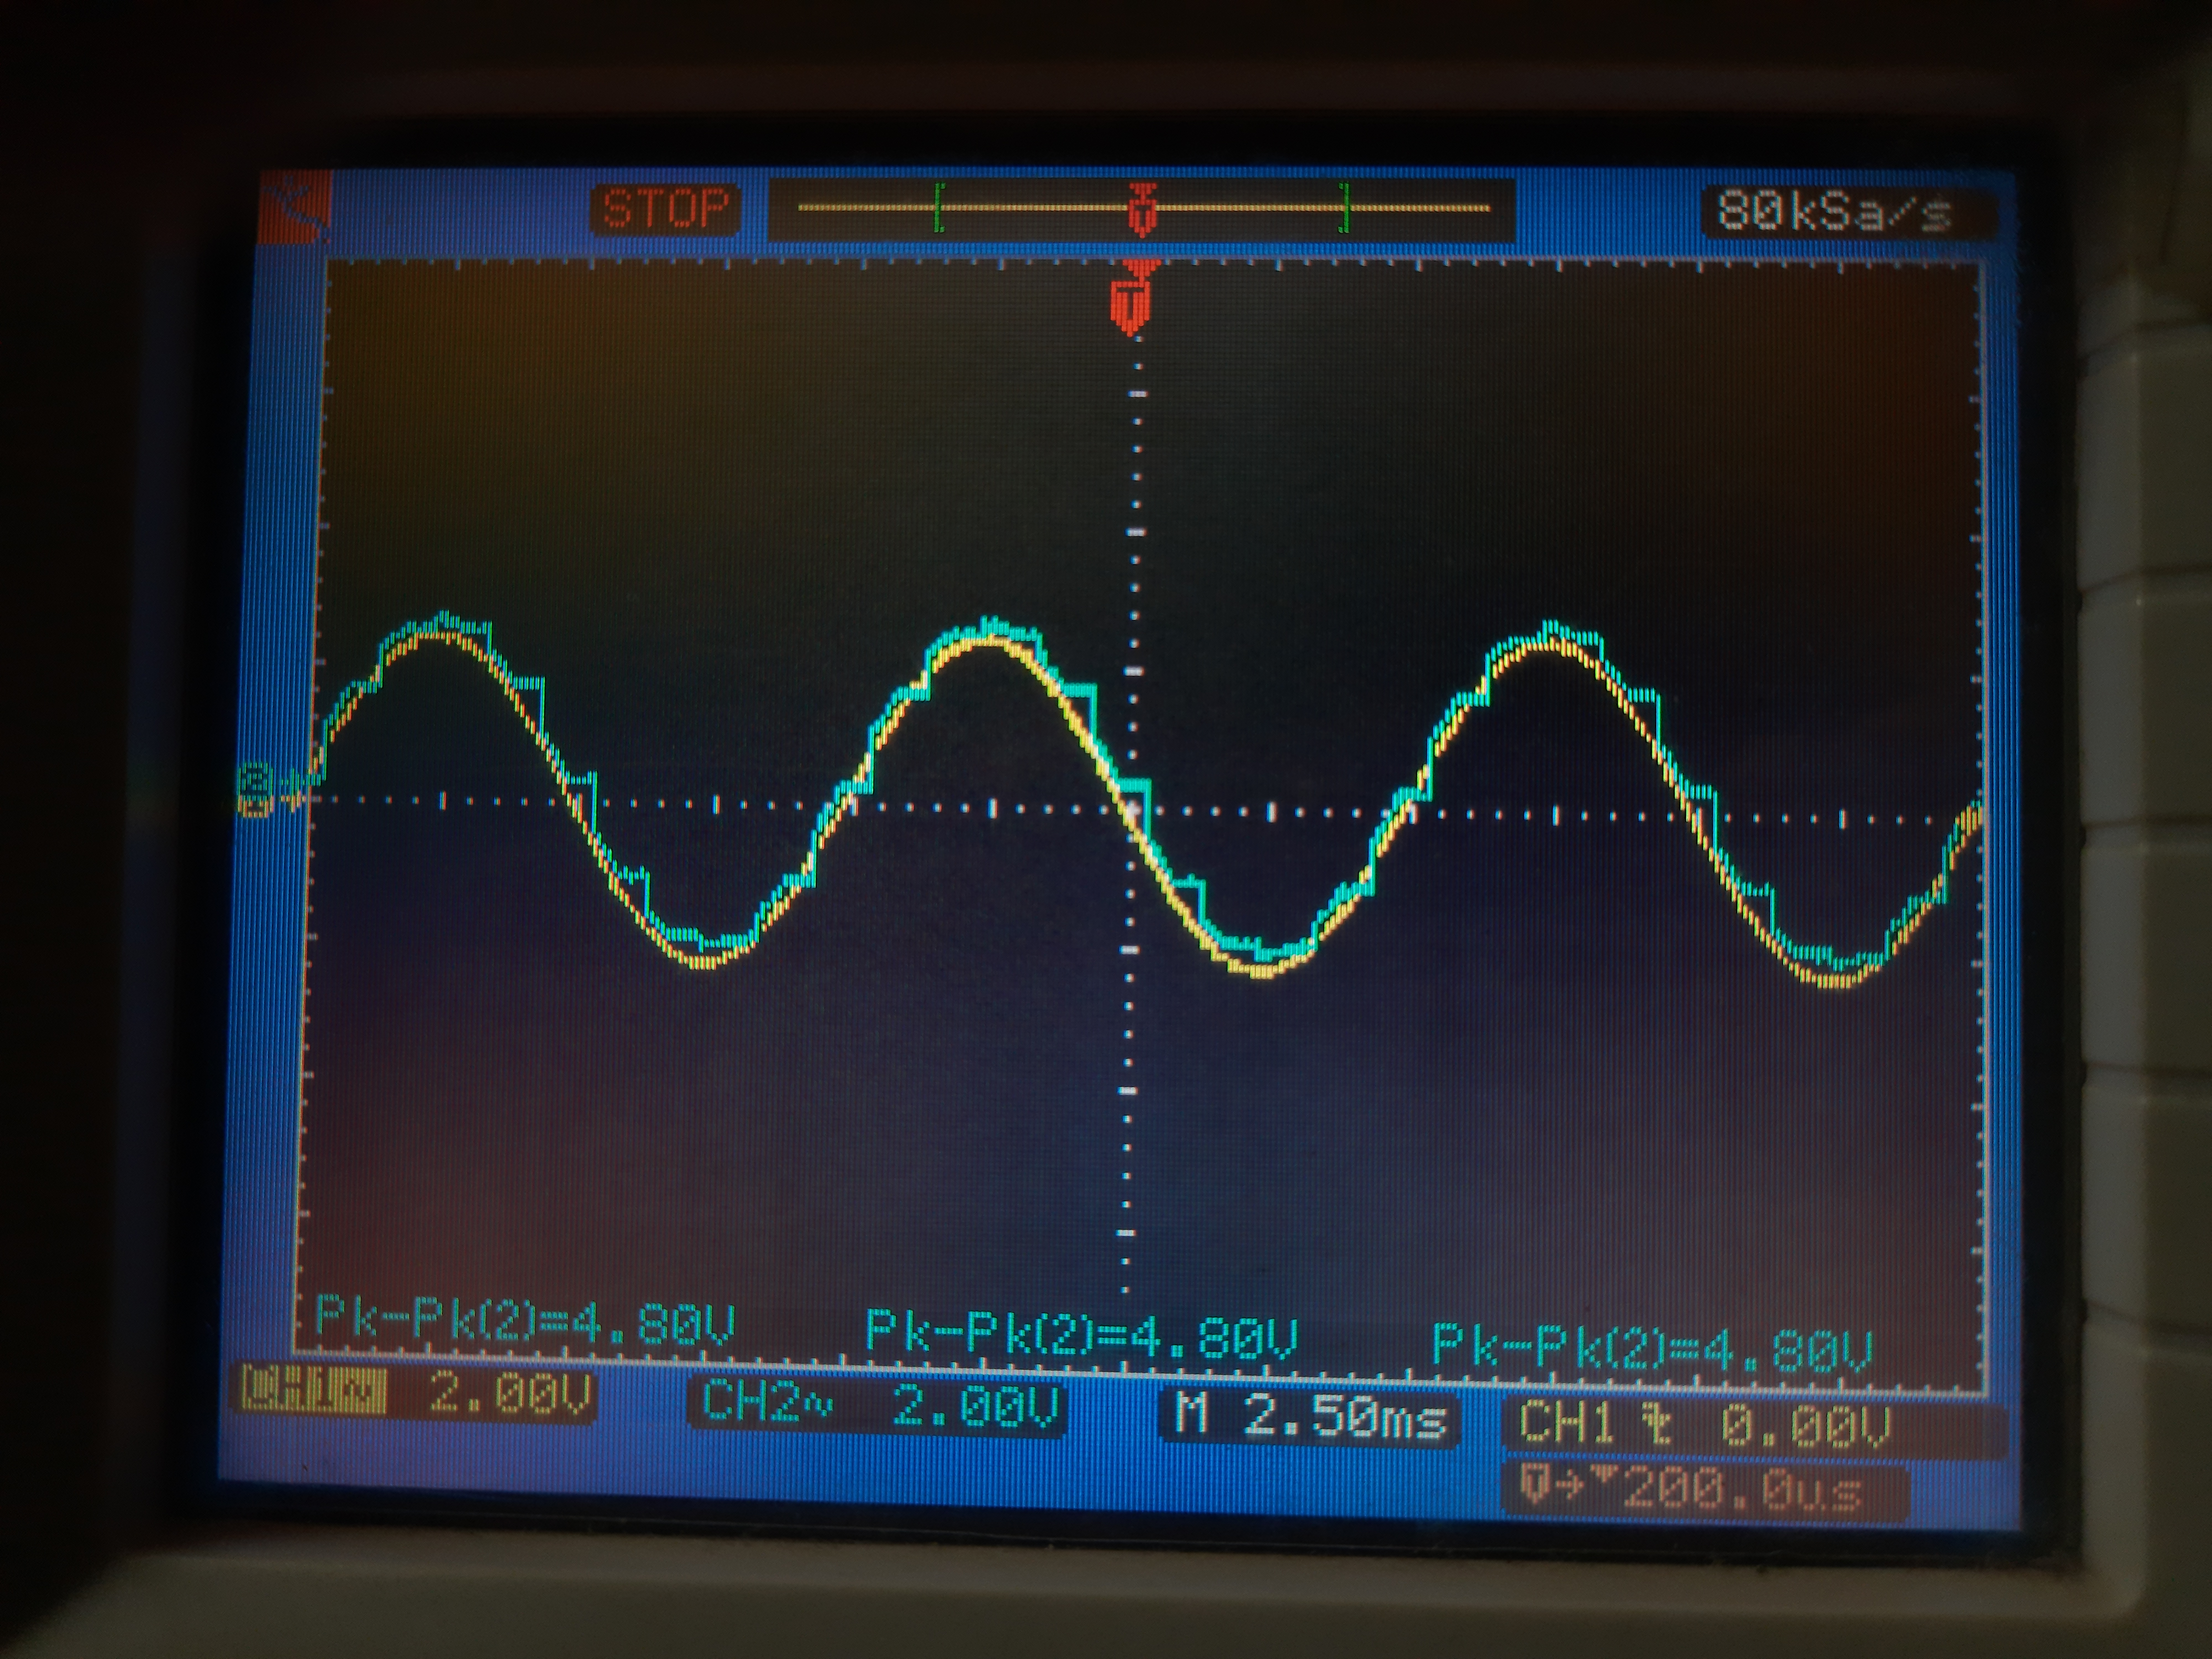
\includegraphics[scale=0.56]{s} 
	\caption{A coincidence spectrum.}
	\label{s}
\end{figure*}


For each angle, time taken to get the coincidence count was set to 3600 s. The angles taken were 180, 90, 175 and 185 degrees.It is seen that maximum coincidence count was seen in 180 degrees arrangement of detectors and almost nil at 90 degrees. For 175 and 185 degrees, a relative lower value than 180 degree arrangement is obtained. 
 
\section{Conclusion}
In the any of the graph three peaks are prominently visible (due to photo peak of $^{22}\text{Na}$, de-excitation of $^{22}\text{Ne}$ and other due to electrical noise) The peak of $^{22}\text{Na}$ was calibrated at 511 keV and the value of the 22Ne peak was obtained at 1275 keV. There is a sharp peak at the starting as there are other peaks which do not occur due to the gamma ray emission(such as electric noise etc).
In the relation between angle and counts per second we observe that it is maximum at 180 degrees and gradually decreases to 0 at ± 90 degrees. Theoretically, if only photo peaks were produced all counts will occurs at 180 degrees and no count at any other degrees (giving a delta peak). However, due to Compton effect and similar effects(back-scattering ,Bremsstrahlung), we observe a distribution curve.
In the 3d heat maps of 185,175,180 \& 90 we observe 4 prominent peaks. However, in the heat map of 90 degrees we observe multiple photo-peaks as Compton effect and bremsstrahlung is observed more.

The sources of error could be improper arrangement of detectors, loose connections of detectors to the computer. Compton scattering back scattering is regarded as noise and ignored. It is to be noticed that many background source radiation may also affect the quality of coincidence counts. Faulty computers (virus infected) should not be used as they may cause data loss and time consumption, as in this experiment. The detectors should be handled carefully and one should not interfere with the ongoing experiment.  

\section{References}
\begin{enumerate}
\item{CS spark gamma spectroscopy manual}
\item{\url{https://www.researchgate.net/figure/Simplified-decay-scheme-of-the-radioactive-isotope-22-Na-22-Na-decays-to-the-excited_fig2_292334939}}
\end{enumerate}

\end{document}